\documentclass[11pt]{article}
\usepackage{fancyheadings,multicol}
\usepackage{amsmath,amssymb}
\usepackage{enumitem,bm}
\usepackage{graphicx, float}

%% Custom page layout.
\setlength{\textheight}{\paperheight}
\addtolength{\textheight}{-2in}
\setlength{\topmargin}{-.5in}
\setlength{\headsep}{.5in}
\addtolength{\headsep}{-\headheight}
\setlength{\footskip}{.5in}
\setlength{\textwidth}{\paperwidth}
\addtolength{\textwidth}{-2in}
\setlength{\oddsidemargin}{0in}
\setlength{\evensidemargin}{0in}
\flushbottom

\allowdisplaybreaks

%% Custom headers and footers.
\pagestyle{fancyplain}
\let\headrule=\empty
\let\footrule=\empty
\lhead{\fancyplain{}{Spring 2018}}
\rhead{\fancyplain{}{CSCI-B455: Machine Learning}}
\cfoot{{\thepage/\pageref{EndOfAssignment}}}

%% Macros to generate question and part numbers automatically
\newcounter{totalmarks}
\setcounter{totalmarks}{0}
\newcounter{questionnumber}
\setcounter{questionnumber}{0}
\newcounter{subquestionnumber}[questionnumber]
\setcounter{subquestionnumber}{0}
\renewcommand{\thesubquestionnumber}{(\alph{subquestionnumber})}
\newcommand{\question}[2][]%
  {\ifx\empty#2\empty\else
   \addtocounter{totalmarks}{#2}\refstepcounter{questionnumber}\fi
   \bigskip\noindent\textbf{\Large Question \thequestionnumber. } #1
   {\scshape\ifx\empty#2\empty(continued)\else
   [#2 point\ifnum #2 > 1 s\fi]\fi}\par
   \medskip\noindent\ignorespaces}
\newcommand{\subquestion}[2][]%
  {\ifx\empty#2\empty\else\refstepcounter{subquestionnumber}\fi
   \medskip\textbf{\large \thesubquestionnumber } #1
   {\scshape\ifx\empty#2\empty(continued)\else
   [#2 point\ifnum #2 > 1 s\fi]\fi}
   \smallskip\noindent\ignorespaces}
\newcommand{\bonus}[2][]%
  {\bigskip\noindent\textbf{\Large Bonus. } #1
   {\scshape\ifx\empty#2\empty(continued)\else
   [#2 point\ifnum #2 > 1 s\fi]\fi}\par
   \medskip\noindent\ignorespaces}

% Enable final count to be printed at top
\usepackage{totcount}
\regtotcounter{totalmarks}

\DeclareMathOperator*{\argmax}{arg\,max}

\begin{document}

%\thispagestyle{plain}

\begin{center}
\bfseries
{\Large Homework Assignment \# 2}\\
   Due: Monday, February 19, 2018, 11:59 p.m. \\
   Total Points: \total{totalmarks}
\end{center}

%%%%%%%%%%%%%%%%

%1. %%%%%%%%%%%%%%%%%%%%%%%%%%%%%%%%%%%%%%%%%%%%%%%%%%%%%%%%%%%%%%%%%%%%%
\question{10}
\noindent
Let $X$ have an exponential density
\begin{equation}
f(x|\theta) = 
\left\{
\begin{array}{l l}
    \theta e^{-\theta x},  & \quad \text{if } x \geq 0 \\
    0, & \quad \text{otherwise}\\
\end{array}
\right.
\end{equation}
\noindent
Suppose that $n$ samples $x_1,\dots,x_n$ are drawn independently according to $f(x|\theta)$. Show that the maximum-likelihood estimate for $\theta$ is $\hat{\theta} = \frac{1}{\frac{1}{n}\sum_{k=1}^n x_k}$


\paragraph{}
$f(x;\theta) = \theta e^{-\theta x}$\\
$L(\theta) = argmax\theta e^{-\theta \sum xk}$\\
Taking the log:\\
$logL(\theta) = log\theta - \theta \sum xk$\\
\\
Take derivative:\\
$\frac{1}{\theta} - \sum xk$\\
$\hat{\theta} = \frac{1}{\frac{1}{n}\sum xk}$\\


%2. %%%%%%%%%%%%%%%%%%%%%%%%%%%%%%%%%%%%%%%%%%%%%%%%%%%%%%%%%%%%%%%%%%%%%
\question{10}
Suppose that the number of accidents occurring daily, $x_i$, in a certain plant has a 
Poisson distribution with an unknown mean $\lambda$. So $P(x_i) = \lambda^{x_i} e^{-\lambda}/(x_i!)$.
Based on previous experience in similar industrial plants, 
suppose that our initial feelings about the possible value of $\lambda$ 
can be expressed by an exponential distribution with parameter $\theta=\tfrac{1}{2}$. 
That is, the prior density is
%
\begin{align*}
f(\lambda)=\theta \textrm{e}^{-\theta\lambda}
\end{align*}
%
%
where $\lambda\in (0,\infty)$. 
If there are 79 accidents over the next 9 days, \textbf{determine the maximum a posteriori (MAP) estimate of  $\lambda$}. 


\paragraph{}
$substitute \theta = 0.5$\\
Taking the log:\\
$log0.5 - 0.5\lambda + \sum (xilog\lambda - \lambda - logxi!)$\\
\\
Take derivative:\\
$-0.5 + \frac{1}{\lambda} \sum xi - n = 0$\\
$\lambda = \frac{1}{n + 0.5}\sum xi$\\
$ \lambda = \frac{1}{9+0.5} * 79$\\
$ \lambda = 8.32$
%3. %%%%%%%%%%%%%%%%%%%%%%%%%%%%%%%%%%%%%%%%%%%%%%%%%%%%%%%%%%%%%%%%%%%%%

\question{10}

\noindent
Consider the binary hypothesis testing (Bayesian classification) problem and refer to the following graph (shown below) for the PDF of $Y$ under $H_0$ and $H_1$:

\begin{figure}[htb]
\centering
\centerline{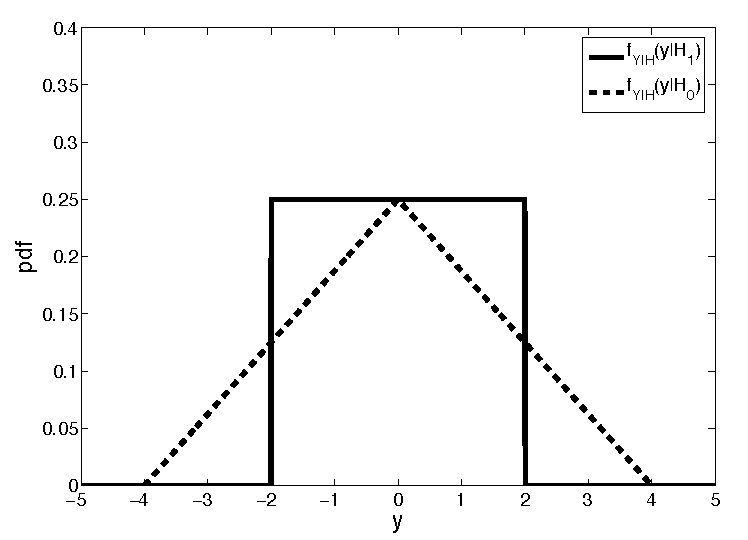
\includegraphics[width=6cm]{bayesdetection.pdf}}
%
\end{figure}

\begin{enumerate}[label=(\alph*)]
\item Using the graph below, write equations (in terms of $y$) for the following likelihoods $f_{Y|H}(y|H_0)$ and  $f_{Y|H}(y|H_1)$
\item For equal priors and uniform costs ($C_{00} = C_{11} = 0$ and $C_{01} = C_{10} = 1$), find the Bayesian decision rule for testing $H_0$ versus $H_1$
\item For part (b), compute the minimum Bayesian risk
\end{enumerate}

\paragraph{}
$3a) fY|H(y|H0) = -\frac{|y|}{16} + 0.25, -4\leq y \leq 4$\\
                         0, otherwise\\
$fY|H(y|H1) = 0.25, -2 \leq y \leq 2$\\
                        0, otherwise\\
\\
$3b) fY|H(y|H0), if -4 \leq y \leq -2, 2 \leq y \leq 4$\\
$fY|H(y|H1), if -2 < y <2$\\ 
\\
$3c)  \frac{1}{2}(\int_{2}^{0} -\frac{1}{16}y + \frac{1}{4}dy + \int_{0}^{-2}\frac{1}{16}y+\frac{1}{4}dy + \frac{1}{2})$\\
$= \frac{1}{2}(-\frac{4}{32} + \frac{2}{4}) + \frac{1}{2}(-(\frac{4}{32}-\frac{2}{4}))$\\
$=0.375 = \frac{3}{8}$
%5. %%%%%%%%%%%%%%%%%%%%%%%%%%%%%%%%%%%%%%%%%%%%%%%%%%%%%%%%%%%%%%%%%%%%%

\question{10}
In this problem, there are 4 binary random variables: G = "gray", V = "Vancouver", R="rain", and S="sad". Consider the directed graphical model, shown below, which describes the relationship between these random variables:

\begin{figure}[H]

\begin{minipage}[b]{1.0\linewidth}
  \centerline{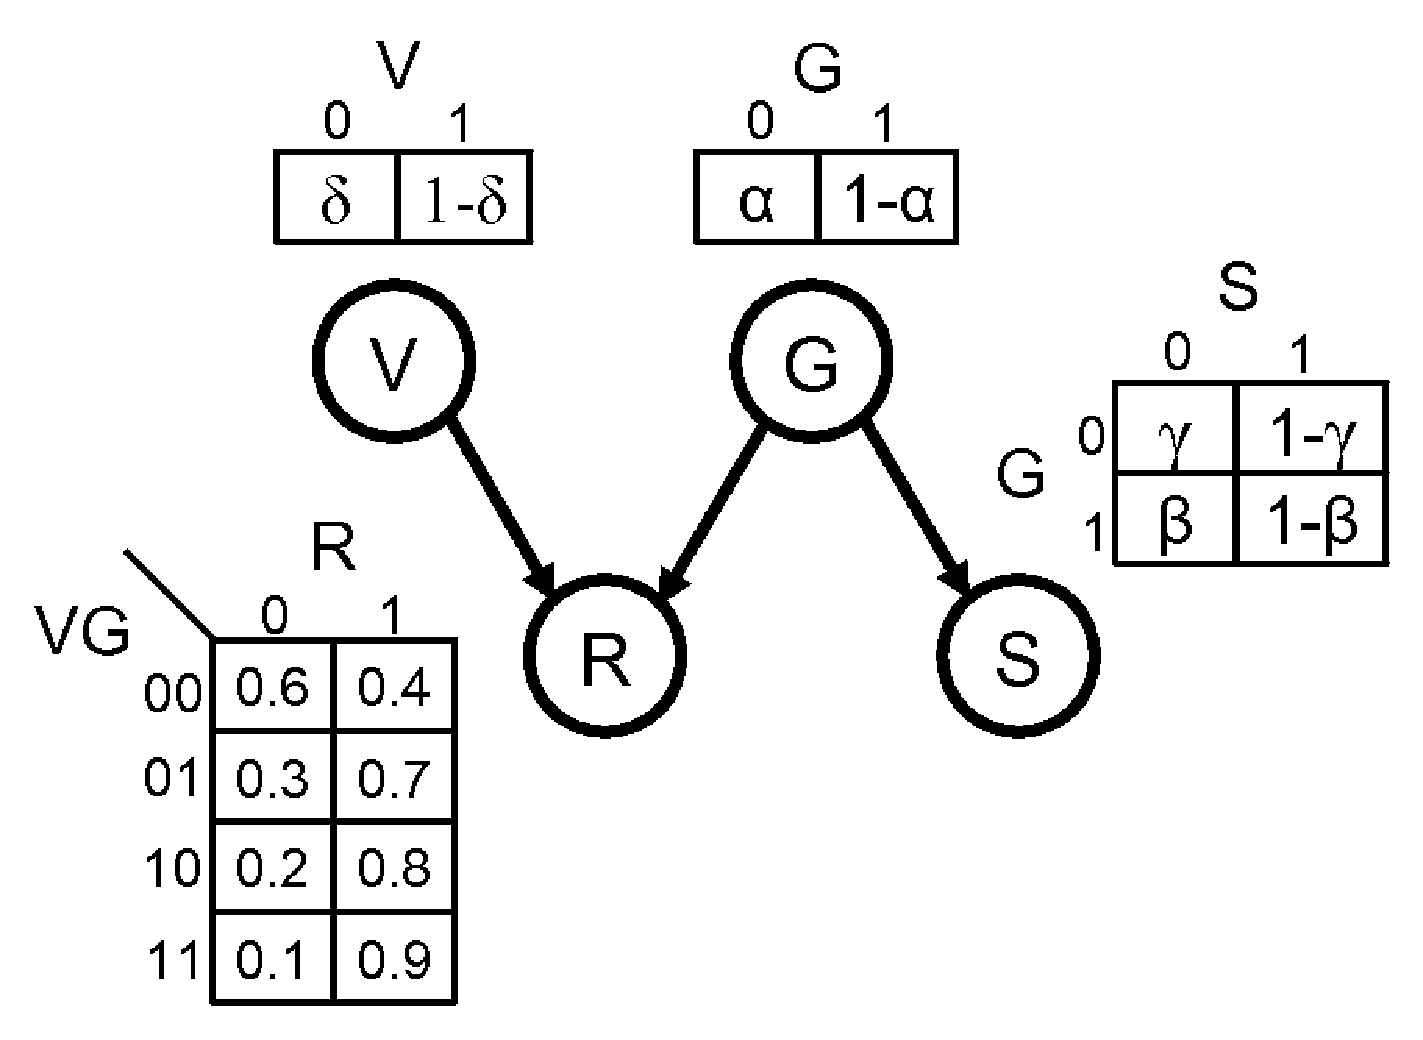
\includegraphics[scale=0.27]{weatherbn.pdf}}
%  \vspace{2.0cm}  
\end{minipage}
\end{figure}


\begin{enumerate}[label=(\alph*)]
\item Write an expression for $P(S=1|V=1)$ in terms of $\alpha, \beta, \gamma, \delta$.
\item Write an expression for $P(S=1|V=0)$. Is this the same or different to $P(S=1|V=1)$? Explain why.
\end{enumerate}

\paragraph{}
4a)$P(S = 1|V = 1) = \frac{((1 - \gamma) + (1 - \beta))(1-\delta)}{1-\delta}$\\
${2 - \gamma - \beta}$\\
4b)$P(S = 1|V = 0) = \frac{((1 - \gamma) + (1 - \beta))(\delta)}{\delta}$\\
$2 - \gamma - \beta$\\
They are the same, because these two are independent events, the result of V does not affect event S.
%%%%% All questions from which to subselect
%\input{assqs/a1_axiom}
%\input{assqs/a1_biaseddie}
%\input{assqs/a1_bonus}
%\input{assqs/a1_bonus2}
%\input{assqs/a1_children}
%\input{assqs/a1_covariance}
%\input{assqs/a1_coin}
%\input{assqs/a1_dice}
%\input{assqs/a1_electrical}
%\input{assqs/a1_expectations}
%\input{assqs/a1_fallacy}
%\input{assqs/a1_figure15xyz}
%\input{assqs/a1_game}
%\input{assqs/a1_median}
%\input{assqs/a1_monty}
%\input{assqs/a1_prove_prob_dist}
%\input{assqs/a1_sumproof}
%\input{assqs/a1_xyz}




% To get the last page number
\label{EndOfAssignment}%

\end{document}
